\documentclass[12pt]{article}
\usepackage[dutch]{babel}

\usepackage{amsmath}
\usepackage{graphicx} 
\usepackage{lscape}
\usepackage{marvosym}
\usepackage{hyperref}
\usepackage[T1]{fontenc}
\usepackage{multirow}


\addtolength{\oddsidemargin}{-.5cm}
\addtolength{\evensidemargin}{-.5cm}
\addtolength{\textwidth}{+1cm}
\addtolength{\topmargin}{-1cm}
\addtolength{\textheight}{+1.5cm}

\begin{document}

\title{Programmeer project\\Connect Four}
\author{Gerwin Puttenstein\\s1487779}
\date{\today}
\maketitle
\newpage
\tableofcontents
\newpage
\section{Inleiding}
Een van de doelen van de afgelopen module, module Software Systemen, was het maken van het project. Als project wordt er een spel gemaakt. Dat spel moet over een server gespeeld kunnen worden en het spel moet zelf controleren of de spelers zich aan de regels houden en of er iemand gewonnen heeft als er een set gedaan is. Het gaat om een bordspel waarbij het niet gaat om geluk maar om strategie zodat er ook een AI voor gemaakt kan worden die door zijn strategie bijna standaard wint.\\
Dit jaar is het spel dat ge\"implementeerd zal worden `vier op een rij'. Dit is een spel voor twee personen. Bij `vier op een rij' is het de bedoeling dat men stenen in een van de zeven rechtopstaande kokers gooit, wanneer een kolom vol is mag hier natuurlijk geen steen meer aan toe gevoegd worden. De spelers doen dit om de beurt en proberen er voor te zorgen dat de andere speler geen vier stenen, horizontaal, verticaal of schuin aansluitend heeft liggen en probeert tegelijkertijd dit wel zelf voor elkaar te krijgen. De eerste die dit lukt heeft gewonnen.\\
Als begin positie is het bord leeg. De persoon die begint is vrij om een rij te kiezen. Ook in elke volgende set is er geen beperking bij het kiezen van de kolom. De rij waarop de steen terecht komt is afhankelijk van het aantal stenen dat er al in die kolom liggen, alle stenen zullen namelijk naar beneden vallen. In het echte spel mag men onderling bepalen wie de eerste set mag doen, in mijn versie van het spel wordt dit door de volgorde waarop de spelers op `play' klikken. Dus de speler die als eerste op 'play' heeft gedrukt mag als eerste beginnen en heeft de rode kleur\\
\newpage 
\section{Bespreking van het totale ontwerp}
\subsection{Klassediagram}
Ik heb voor het overzicht van dit diagram de klassen in packages onderverdeeld. Ze zitten in het diagram in dezelfde package als dat ze in het systeem zijn ingedeeld. Ook heb ik ervoor gekozen om geen methodes in het klassediagram op te nemen, dit komt het overzicht niet ten goede. \\
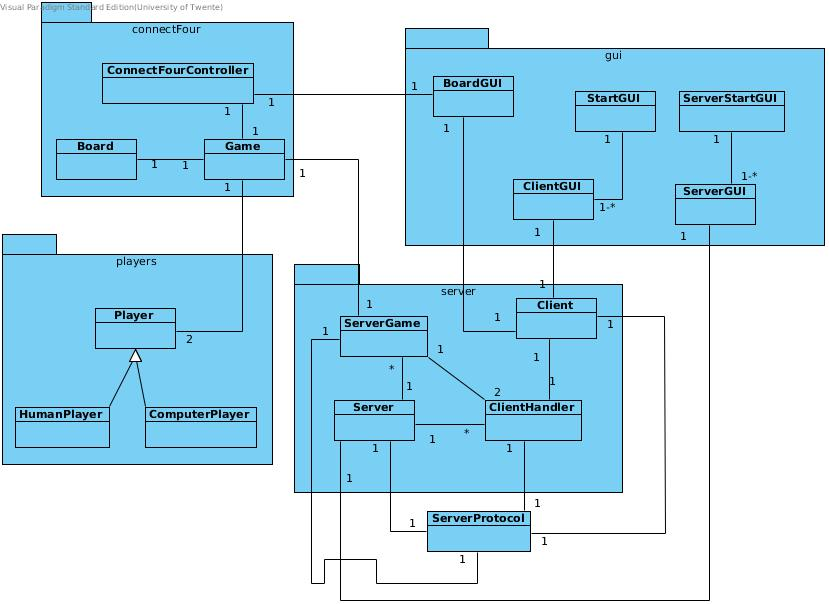
\includegraphics[scale=0.5]{ConnectFour.jpg}\\
De enige klasse die wel in het systeem zit en niet in het klasse diagram is opgenomen is de klasse PlayerColor. Omdat dit een enum is, wordt hij door bijna alle klassen gebruikt en voegt het dus niet veel toe aan het klasse diagram.
\subsection{Vereisten}
Er moesten een aantal belangrijke dingen in het programma komen. Deze staan op pagina 18 van de reader en hier heb ik me dan ook zo goed mogelijk aan gehouden.
Voor de server zijn het de volgende vereisten:
\begin{enumerate}
\item Het poortnummer kan je ingeven via de ServerStartGUI waar de server daarna naar gaat luisteren, mits het een geldig poortnummer is die nog niet in gebruik is.
\item (een goede error wordt gemaakt als port niet kan) Er wordt een error weergeven als er geen geldig poortnummer wordt ingevoerd. Dan terminate het hele programma. 
\item De server ondersteund meerdere games die tegelijkertijd gespeeld kunnen worden. Dit wordt gedaan doordat de Server per twee spelers die willen spelen een nieuwe ServerGame maakt die de Game bij houdt.
\item Er is nu geen TUI die zorgt dat alle berichten naar System.out schrijft, maar een ServerGUI die zorgt dat alle berichten naar een JTextArea worden geschreven die binnenkomen op de server. Ook de berichten die de server stuurt worden naar de JTextArea geschreven.
\item Het serverprotocol dat is besproken tijdens de projectmeeting wordt gerespecteerd. Er zijn een aantal commandos die de server niet kent, en niet alle errors worden gestuurd. De niet ge\"implementeerde commandos hebben te maken met het challenge en leaderboard gedeelte. Dit ondersteund mijn server niet, dus is het ook niet nuttig om deze te implementeren. Ook worden niet alle errors verzonden omdat niet op alles wordt gecheckt.
\end{enumerate}
Voor de client zijn het de volgende eisen die worden gesteld en op de volgende manier zijn ge\"implementeerd.
\begin{enumerate}
 \item Ook hier wordt geen gebruik gemaakt van een TUI, maar van een GUI. Hier is het mogelijk om het adres en de poortnummer van de server waar je op wil spelen kan invoeren en waar je een naam kan invoeren. Ook is het mogelijk om binnen deze GUI te kiezen om standalone te spelen. Dit is een spel tegen de computer.
 \item Er is support voor HumanPlayers en voor ComputerPlayers. Deze maken beide gebruik van een abstracte klasse Player. Hiervoor heb ik een beetje de klassen gevolgd die we hebben gebruikt voor de opdrachen en zelf wat aangepast zodat het beter aansluit op mijn implementatie. De ComputerPlayer bevat een kleine mate van intelligentie, dit houdt in dat de ComputerPlayer een random getal kiest tussen 0 en 6 voor de kolom waar hij een steen wil plaatsen. Er kan online alleen worden gespeeld met een HumanPlayer, de optie om een ComputerPlayer te kiezen is er niet. De ComputerPlayer wordt gebruikt als er standalone wordt gespeeld.
 \item Omdat de ComputerPlayer alleen wordt gebruikt tijdens het standalone spelen en ik gefocust was op het online gedeelte heb ik niet gedacht aan de mogelijkheid om de denktijd van een ComputerPlayer te kunnen veranderen.
 \item Er is een hintsysteem ge\"implementeerd, echter werkt deze niet naar behoren. Hij maakt gebruik van de determineMove() van de ComputerPlayer. Het probleem is dat er niet wordt gekeken of de velden eronder vrij zijn of niet en er wordt dan dus altijd een vakje grijs gekleurd op de onderste rij.
 \item Nadat een client spel heeft gespeeld kan deze gelijk weer een nieuw spel starten door opnieuw op play te drukken.
 \item Als de server onverwachts disconnect dan handelt de client dit goed af. Hij heeft door als er geen connectie meer is en sluit dan veilig alle verbindingen die openstaan. Dan sluit de gui af en termineert het programma.
 \item De client respecteert ook het protocol dat is afgesproken. Ook hier geld dat de leaderboard en challenge commandos niet zijn ge\"implementeerd omdat de client deze niet ondersteund. En er wordt niet veel gedaan met de error commandos die zijn afgesproken.
\end{enumerate}

\subsection{Observer en Model-View-Controller}
Binnen mijn implementatie van het spel is de BoardGUI de observer en de Game klasse de Observable. Wanneer er een zet wordt gedaan op de gui, wordt deze doorgespeeld naar de Game, deze kijkt of dit een geldige zet is en speelt deze zet op het bord, als de zet geldig is. Daarna stuurt de Game een update naar alle Observers. In dit geval is dit alleen de BoardGUI. Als deze een update binnenkrijgt, wordt de zet gedaan op de gui.\\
Ook maak ik gebruikt van het MVC patroon. Binnen mijn implementatie is de Game klasse de model, de BoardGUI klasse de view en de ConnectFourController de controller. De controller maakt een view en een model aan en zorgt ervoor dat updates op de view worden doorgespeeld naar de model en vice versa.

\subsection{Formats voor data opslag en communicatieprotocol}
Een board klasse houdt bij welke plaatsen op het bord zijn bezet met stenen en welke plaatsen nog leeg zijn. Deze velden worden bijgehouden in een array van PlayerColors. Deze array is 42 plaatsen groot, gelijk aan het aantal velden van een vier op een rij spel. Een veld kan leeg zijn, PlayerColor.EMPTY, geel zijn, PlayerColor.YELLOW, of rood zijn, PlayerColor.RED. \\
Voor een online spel houdt een ServerGame bij welke spelers in dat specifieke spel zitten en wie er aan de beurt is. Een ServerGame wordt aangemaakt door de Server als twee spelers willen spelen.\\
Voor het commmunicatieprotocol wordt het protocol gebruikt dat is opgesteld tijdens een projectmeeting. Daar hebben we gekozen om een klasse te gebruiken die commands voor de server, commands voor de client, commands voor beide en errormessages bevat.

\newpage

\section{Discussie per klasse}
Hier volgt een korte toelichting op elke klasse die in mijn implementatie van het spel zitten, opgedeeld per package.\\
\subsection{connectFour}
In deze package zitten alle klassen die nodig zijn voor de kern van het spel.
\subsubsection{Board}
Deze klasse houdt voor elk spel de stand van het bord bij. Ook worden binnen deze klasse de spelregels bijgehouden en zijn er de methoden om te kijken of er een winnaar is. Deze klasse houdt bij of het bord vol is, of het spel voorbij is en wie de winnaar is. \\
De klasse Game gebruik de Boardklasse om het bord aan te kunnen passen, een winnaar te bepalen en te kijken of het spel over is.

\subsubsection{ConnectFourController}
De controller klasse van het spel. Deze klasse maakt een View en een Model aan en zorgt er daarna voor dat er een spel gespeeld kan worden via het MVC patroon. De klasse bevat alleen een contructor om alles aan te maken en een actionPerformed om het klikken op een knop af te handelen.\\
Deze klasse wordt aangeroepen als je standalone wil gaan spelen.

\subsubsection{Game}
De model in het MVC patroon. Deze klasse zorgt ervoor dat er een nieuw spel kan worden gemaakt met twee spelers. Daarnaast houdt hij bij wie er aan de beurt is en voert hij beurten uit voor spelers op een Gui en een bord.\\
De Game wordt aangeroepen door de bovengenoemde controller en door een ServerGame. 

\subsection{gui}
Binnen deze package zijn alle klassen te vinden die zorgen voor het grafische deel van het programma.
\subsubsection{BoardGUI}
De grafische weergave van een bord en tevens de View in het MVC patroon. De BoardGUI bevat in de initi\"ele staat 42 zwarte, niet klikbare knoppen. Deze stellen de velden van een vier op een rij spel voor. Boven elke kolom is een klikbare knop te vinden om een zet te kunnen doen in die kolom.\\
Deze klasse wordt door elke klasse gebruikt die een grafische interface wil voor een bord. 
\subsubsection{ClientGUI}
De GUI die de client te zien krijgt nadat hij connectie heeft gemaakt met de server. Hier kan hij kiezen om te spelen of om te stopppen. Daarnaast kan hij een bericht intypen zodat hij kan chatten. Op een JTextArea worden alle binnenkomende en uitgaande berichten weergeven.\\
Deze klasse wordt alleen door de startgui gebruikt om een nieuwe client te starten. De Client dient als controller voor deze klasse. Deze zorgt ervoor dat de knoppen een functie krijgen en dat de JTextArea wordt geupdate.
\subsubsection{ServerGUI}
De GUI die men te zien krijgt als er een server is gestart vanaf de ServerStartGUI. Op de GUI zijn twee JTextAreas. Op de ene staan alle binnenkomende en uitgaande berichten van de server. Op de ander staat een lijst van clientnamen die geconnect zijn met de server.\\
Deze GUI wordt gestart door een ServerStartGUI. De ServerGUI zorgt ervoor dat er een Server wordt gestart. De Server is de controller voor deze klasse en zorgt ervoor dat de JTextAreas worden geupdate.
\subsubsection{ServerStartGUI}
De ServerStartGUI zorgt ervoor dat er een poortnummer kan worden ingevoerd en dat er een server kan worden gestart. Deze GUI bevat slechts een JTextField en een JButton. De textfield om een poortnummer in te kunnen voeren en de button om een server te starten. Als de poortnummer niet geldig is termineert het programma.\\
Deze klasse is van geen andere klasse afhankelijk. Hij start alleen een server, mits het ingevoerde poortnummer is geldig.
\subsubsection{StartGUI}
Met de startgui kan een nieuwe client worden gestart of kan er standalone worden gespeeld. Als men standalone wil spelen hoeft er niks te worden ingevuld, maar mocht men dit willen kan er een naam worden ingevuld. Als men een client wil starten en dus online wil spelen moeten alle velden worden ingevoerd. Deze zijn er een voor de naam, een voor het ipadres en een voor de poortnummer. Als al deze waarden geldig zijn en ingevuld wordt er een nieuwe client gestart en connectie gemaakt met de server, mits deze server bestaat op de gegeven waarden.\\
De StartGUI kan los gedraaid worden en heeft geen andere klassen nodig om te werken. Een inner klasse zorgt ervoor dat de knoppen functies krijgen en dat de ingevoerde informatie wordt gecheckt en verwerkt.

\subsection{Players}
Binnen deze package zijn drie klasses. Twee klasses extenden de derde klasse.
\subsubsection{Player}
De abstracte klasse binnen deze package. Deze heeft de methodes die elke Player nodig heeft, zoals een getName() of getColor(). Er is een abstracte methode binnen de klasse. Deze verschilt dus per extentie van Player. 
\subsubsection{HumanPlayer}
Een extentie van Player. Deze klasse heeft niet veel meer functie in het spel dan de naam en de kleur van de speler bijhouden.\\
Deze klasse heeft dus Player nodig, omdat hij Player extend.
\subsubsection{ComputerPlayer}
Een tweede extentie van Player. Dit keer is het een ComputerPlayer. Deze heeft een zekere vorm van AI. De klasse wordt gebruikt om zetten te doen zonder dat daar een mens voor nodig is. Als iemand standalone kiest op de StartGUI, dan gaat hij spelen tegen een ComputerPlayer.\\
De ComputerPlayer neemt een random getal tussen de 0 en de 6 en doet in die kolom een zet.\\
Ook deze klasse is afhankelijk van Player, omdat hij Player extend.
\subsection{server}
Binnen deze package zijn alles klasses die te maken hebben met de Client-Server connectie en het spelen van een spel via een server.
\subsubsection{Client}
De Client zorgt ervoor dat een persoon verbinding kan maken met een server met berichten kan sturen naar de server. Een Client zorgt er ook voor dat de berichten die binnen komen goed worden verwerkt.\\
De Client is afhankelijk van een ClientHandler om daadwerkelijk met een server te kunnen communiceren.
\subsubsection{ClientHandler}
De ClientHandler is een klasse die wordt gestart als een Client een connectie wil met de Server. De Server maakt dan bij een binnenkomend verzoek een nieuwe ClientHandler aan. Deze ClientHandler zorgt er voor dat berichten die gestuurd worden vanaf de Client naar de Server worden afgehandeld. Dus als bijvoorbeeld een Client het commando play stuurt, dan krijgt de ClientHandler dit bericht en zorgt dan dat de server hier dingen mee gaat doen, in dit geval de Client in een wachtrij stoppen of als er genoeg spelers zijn, in een spel stopppen.
\subsubsection{Server}
De Server zorgt ervoor dat Clients met elkaar kunnen communiceren. Hier maken alle Clients mee verbinding en via de Server worden dan de berichten verspreid, of worden nieuwe spellen gestart of gestopt. 
\subsubsection{ServerGame}
De ServerGame klasse houdt een spel bij die op de Server draait. Binnen deze klasse zijn twee ClientHandlers geregistreerd die met elkaar een spel aan het spelen zijn. Een Server maakt een nieuwe ServerGame aan per twee ClientHandlers die hebben aangegeven dat ze een spel willen spelen. Binnen de ServerGame worden de binnenkomende moves gecheckt en wordt er na elke move gekeken of er al een winnaar is of dat het spel al voorbij is. Dan stuurt een ServerGame via de Server de moves of een game over naar de verbonden ClientHandlers die in dit spel zitten.\\
Per Server kunnen er meerdere ServerGames zijn, dit zorgt er dan voor dat er meerdere spellen tegelijkertijd gespeeld kunnen worden op een Server.

\subsection{tests}
De test klassen die in deze package te vinden zijn worden besproken in het gedeelte over de tests.

\subsection{utils}
Binnen deze package zijn een aantal klassen die door een aantal andere klassen worden gebruikt zonder verder invloed te hebben op uitkomsten of hoe het eruit ziet.
\subsubsection{PlayerColor}
Een enum klasse. De enum bestaat uit drie delen, namelijk een RED, een YELLOW en EMPTY. Met deze enum wordt er binnen het spel aangegeven welke kleur een veld heeft en welke kleur een speler is. Voor een veld kan dat RED, YELLOW of EMPTY zijn, waar RED een rood veldje voorsteld, YELLOW een geel veldje en EMPTY een leeg veldje.
\subsubsection{ServerProtocol}
Deze klasse hebben we tijdens een projectmeeting opgesteld toen we het protocol gingen samenstellen. Binnen deze klasse zijn een aantal final Strings die commandos voorstellen voor de Client-Server commmunicatie. Hier moeten zowel de Client als de Server zich aan houden.Dit protocol zorgt er ook voor dat verschillende implementaties van het spel toch tegen elkaar kunnen spelen.

\section{Testrapport}
Het testen van het systeem ging op verschillende manieren. Omdat er veel gebruik wordt gemaakt van GUIs, worden deze getest door te kijken of alles binnen de GUI werkt en goed reageert op invloeden van buiten. Ook is het voor de GUIs belangrijk dat ze goed in elkaar zitten en niet raar er uit zien.\\
\subsection{GUI test}
Per GUI heb ik gekeken wat er gebeurde als ik bepaalde knoppen in drukte of wat er met een JTextArea gebeurde als er een nieuw bericht werd gegenereerd.
\subsubsection{BoardGUI}
Voor de BoardGUI is het belangrijk dat de knoppen boven de kolommen goed werken en de juiste events genereren. Dit heb ik gedaan door een nieuw spel te starten en gewoon te gaan spelen. Door op een knop te drukken werd dan een steen geplaatst in de juiste kolom en werd deze zo ver mogelijk naar onderen geplaatst.\\
Ook was belangrijk dat de knoppen die de velden moeten voorstellen juist werden gekleurt. Dit gebeurde ook als de knop boven de desbetreffende kolom werd ingedrukt en werkte dit gedeelte ook naar behoren. Het enige gevaar was nog als de rij vol was en je wil nog een steen daar plaatsen. Hier kwam ik tijdens het spelen achter. Dit is opgelost door een bericht te geven dat je hier geen steen mag plaatsen en dan het programma te termineren, zoals ook is afgesproken in het protocol.\\
Dit werkte goed in een standalone versie van het spel, alleen tijdens het testen van het systeem kwam ik er achter dat als een kolom helemaal wordt gevuld en er komt nog een steen bij dat niet de Client maar de Server stopt. Dus dan stopt iedereen. Dit is logisch, omdat de Game wordt gemaakt op de Server en de Game een move checkt. Maar dit zou doorgespeeld moeten worden naar de Client. \\
Na deze test heb ik dit veranderd en wordt het te spelen field -1, zodat hier op gecheckt kan worden en er een invalid move gestuurd kan worden als de move niet valid is.
\subsubsection{ClientGUI}
Wat hier getest moest worden was of het logpanel goed werd geupdate met berichten die binnenkwamen en eruit gingen en dat de knoppen "play" en "quit" werkten.\\
Het logpanel is getest door te kijken naar de berichten die op de console van eclipse stonden en deze te vergelijken met de berichten in het logpanel. Deze kwamen altijd over een en concludeerde ik dat de berichten goed werden weergeven.\\
De knoppen werden getest door er op te klikken en kijken wat de uitkomst was. Voor "play" zou dit moeten zijn dat er een play wordt verstuurd naar de server. Dit werd gedaan en als er nog een andere speler dit had gedaan werd er een nieuw spel gestart.\\
Voor "quit" geld dat de socket goed wordt afgesloten en dat de gui verdwijnt. Dit wordt goed gedaan omdat de Server weet dat een Client is geleaved als een Client op quit drukt.
\subsubsection{ServerGUI}
Voor de ServerGUI geldt ongeveer hetzelfde als voor de ClientgUI. Het logpanel en het clientpanel moeten de juiste informatie weergeven. Dit heb ik op dezelfde manier getest als bij de Client en dit gaat goed.\\
Bij de ServerGUI heb ik ook een panel waar een lijst staat met Clients. Deze wordt ook goed geupdate. Dit heb ik getest door Clients te connecten en te verwijderen van de Server. Ten allen tijde klopte de lijst met de Clients die waren geconnect.\\
Er was een probleem, en dat was dat twee Clients dezelfde naam hadden, dit zou niet mogen kunnen, maar er wordt niet op gecheckt door de Server. Dus als een van de twee van de Server disconnect verdwijnen beide namen uit de lijst, terwijl er nog wel een van de twee is geconnect.\\
Een ander probleem wat er is met de ServerGUI is dat als ik de GUI sluit, de server door blijft draaien tot ik deze handmatig termineer via de console van eclipe. Ik ben nog niet achter de oorzaak hiervan gekomen.
\subsubsection{ServerStartGUI}
Hier gaat het er vooral om dat de informatie die wordt ingevoerd geldig is en dat de knop een nieuwe server start. Dit is makkelijk te testen door dingen in te voeren en een server te starten.\\
Dit geeft als resultaat dat als er geen nummer wordt ingevoerd dit wordt gemeld en het programma wordt gestopt.\\
Echter als het poortnummer in gebruik is, wordt er toch geprobeerd een nieuwe server te starten en dan wordt er dan toch een error gecre\"erd dat er een nullpointer is omdat de Socket niet geopend kon worden.
\subsubsection{StartGUI}
Ook hier geld dat de informatie die wordt ingevoerd goed moet worden gecheckt en moet worden afgehandeld als de informatie niet klopt. Zolang een Client niks met de informatie kan die is ingevoerd en er wordt toch geprobeerd verbinding te maken met een niet bestaande server wordt het programma simpelweg gestopt.\\
Voor de knoppen gaat het erom dat voor de een een standalone spel wordt gestart en voor de ander er word geprobeerd verbinding te maken met de server. Dit wordt correct gedaan.
\subsection{connectFour package}
De Board klasse is getest door een test klasse te schrijven, namelijk testBoard. Deze klasse maakt gebruik van JUnit om te testen. Per test staat er een stukje commentaar bij wat er precies wordt getest. Dit was goed om te doen, omdat er binnen de Board klasse de spelregels zijn ge\"implementeerd. De test gaf geen errors en dus kloppen alle methods. De testBoard gaf op de Board een coverage van 90.4\%.\\
De Game klasse is lastig te testen, omdat deze erg afhankelijk is van andere klassen. Dus hiervoor heb ik een nieuwe standalone spel gestart en gekeken of de Game goed reageerde op de input die ik gaf. Het enige waar deze dus niet goed op reageerde was als de kolom vol was. Dan wordt in multiplayer de Server gestopt. Dit is licht veranderd zodat de server en in ieder geval niet meer mee stopt.

\subsection{Player package}
Voor de Player package heb ik een nieuwe JUnit test case gemaakt die alle drie de klassen in de package test. Dit kan omdat twee klassen, namelijk ComputerPlayer en HumanPlayer, extenties zijn van Player.\\
Deze testklasse geeft voor ComputerPlayer en HumanPlayer een coverage van 100\% en voor Player een coverage van 62.5\%.

\subsection{Server package}
Het server gedeelte is wat lastiger te testen omdat de klassen elkaar nodig hebben om te testen. De server was hiervan nog het makkelijkste om te testen door verbinding te maken met telnet en commandos te sturen naar de server om te kijken of deze correct reageerd.\\
Hier ben ik erachter gekomen dat de server altijd correct terug reageerd. Als ik bijvoorbeeld een niet bestaand commando geef, dan krijg ik een Invalid Command error terug en als ik chat en bericht doe, dan chat ik op de server.\\
Via dit test je ook of de Client goed communiceerd. Dus of de juiste commandos het juiste effect hebben op de server. Het spelen van een spel werkt niet correct via een telnet, omdat hier een GUI voor nodig is om correct te functioneren. Via telnet kan je zetten blijven spelen, ook al ben je niet aan de beurt. Via de GUI wordt dit geregeld door knoppen te disablen als je niet aan de beurt bent.\\
De Client-Server gedeelte wordt verder getest in een system test.

\subsection{System tests}
In deze sectie zal ik kort beschrijven hoe ik de requirements heb getest in het systeem.\\
Eerst heb ik een gewone run gedaan door het programma, dus een server gestart, hier een client mee verbonden en gekeken of dit goed ging. Hier gebeurde niks raars, dus een tweede Client laten connecten. Nu ziten er twee clients in de server en kan er dus een spel gespeeld worden. Dus een spel gestart en deze uitgespeeld. Het spel werd correct afgesloten en er werd vermeld wie de winnaar was. \\
Na dit spel heb ik een client een chatbericht laten sturen om te kijken of deze aan kwam. Dit ging goed en gaf geen onverwachte dingen.\\
Een client verwijderd en een nieuwe client gestart. Toen heb ik met de eerste client en de nieuwe client een nieuw spel gestart. Dit was mogelijk en een tweede spel gespeeld. Hierna beide clients laten disconnecten en de server gestopt.\\
Nu een client gestart met foute informatie, dit zorgde ervoor dat het programma werd getermineert, zoals verwacht.\\
Nu doen we dit ook voor de Server. Dus we voeren een poortnummer in dat geen getal is. Dan termineert het programma met het bericht: NaN. Als we hier een poortnummer invoeren dat wel een nummer is maar niet geldig is, bijvoorbeeld 454545. Dan zou het mogelijk moeten zijn om een nieuw poortnummer in te voeren met een melding dat het ingevoerde poortnummer niet een mogelijk poortnummer was. Dit gebeurt niet, er wordt een exceptie gegooit die nergens wordt opgevangen. Het programma termineert dan niet en blijft draaien. Dit is niet het gewenste resultaat.\\
Voor de Server moet het mogelijk zijn om meerdere spellen tegelijkertijd te ondersteunen. Hiervoor starten we 4 Clients en registeren we die op dezelfde server. Dan laten we alle clients op play drukken. Dan worden er twee ServerGames gecre\"eerd door de Server, wat betekend dat er twee spellen worden gestart. Er worden dan ook 4 BoardGUIs gestart. Hier is te zien dat er twee spellen zijn, omdat een Client maar een andere Client be\"invloed en niet allemaal.\\
Het protocol van de server heb ik getest door een telnet te starten en deze te laten verbinden met de server. De server reageert correct op de afgesproken commandos. Echter als er een niet geldig commando wordt ingevoerd, wordt er wel een invalidCommand error gestuurd, maar hier wordt verder niks mee gedaan. Dit probleem ligt bij de Client.\\
Een client moet correct reageren wanneer een server er plotseling mee stopt, dus wanneer de verbinding tussen de Client en de Server door de Server wordt verbroken. Hiervoor start ik een Server en een Client. Dan stop ik de Server. De Client geeft dan het bericht dat de verbinding tot de server is verloren en dat het client programma wordt getermineert. Dit is het verwachte resultaat van een Client.

\section{Metrics report}
Voor de analyse van mijn code met de Metrics plugin heb ik eerst gekeken naar de MLoC(Method lines of code). Hiervoor heb ik een klein experiment gedaan met een aantal methodes binnen mijn systeem. Hieruit heb ik geconcludeerd dat mijn code een goede kwaliteit heeft, omdat de MLoC zo klein mogelijk is. Zo start ik bijvoorbeeld een else gelijk na het haakje van een if in plaats van op een nieuwe regel. Door dit een aantal keer in een methode te doen daalt de MLoC.\\
Voor de cyclomatic complexity van mijn code heb ik een aantal methodes binnen een aantal klassen die zeer hoog uitvallen. Dit zijn met name de run methodes voor de Server en de Client, omdat deze een oneindige while loop bevatten. Ook binnen de board zijn er een aantal hoge waarden. Deze zijn voor het tellen van de stenen voor een winnaar. Dit komt omdat ik een aantal loops in elkaar heb en daar binnen weer een if-elseif contructie. Dit geeft hoge waardes. Dit komt mijn kwaliteit van de code niet ten goede, maar dit is nu eenmaal de manier voor mij om dit te doen. Ik zie geen andere mogelijkheid om dit te maken.\\
Daarnaast heb ik ook nog naar de weigthed methods per class gekeken. Deze was voor een aantal klassen zeer hoog. Dit komt door het aantal for loops en if statements die er in deze klassen te vinden zijn. Deze hoge waarden houden in dat de klassen applicatiespecifiek zijn. Voor bijvoorbeeld Board, met een WMC van 84, klopt dit ook. Hier zijn de spelregels voor Vier op een rij en dus is deze klasse niet echt voor een andere applicatie te gebruiken. De GUIs hebben een vrij lage waarde, dus deze zijn wat makkelijker te hergebruiken.\\
Al met al is de code niet overal van goede kwaliteit en niet altijd even herbruikbaar. De MLoC waren wel mooie waren die zo laag mogelijk waren. Echter waren de cyclomatic complexity en de WMC vrij hoog. Dit zou nog naar beneden kunnen om de kwaliteit van de klassen te kunnen verbeteren.

\section{Reflectie op de planning}
\subsection{Ervaringen week vier}
In de vierde week van de module zijn we in het design project gaan kijken naar wat er zoal gedaan moest worden en hoeveel tijd de losse onderdelen zouden gaan kosten. Ook hebben we gekeken naar welke dingen eerst af moesten voor we verder konden. Dit is mij erg van pas gekomen bij het plannen van mijn programmeer project. Sommige dingen, zoals het uitbreiden van de GUI bijvoorbeeld had ik heeft veel zin in maar heb ik toch nog aan de kant geschoven om eerst de verplichtte vereiste af te krijgen. Daarom heb ik de vereisten boven aan gezet en ben ik daarna gaan kijken naar de extra's die ik nog kon implementeren.\\
\subsection{Project planning}
Tijdens de projectweken van de tweede module waar ik eigenlijk deze opdracht moest afhebben was het me niet gelukt om me aan mijn planning te houden. Dit door andere dingen die onverwachts meer tijd nodig hadden.\\
Omdat ik nu deze opdracht heb gerepareerd in een andere module, was het extreem belangrijk dat ik me aan mijn planning hield. Dit is me dan ook beter gelukt dan in het begin.  Soms heb ik echter wel moeten afwijken van mijn planning omdat er dan dingen zijn die onverwachts weer meer tijd kosten of een opdracht van de andere module die wat meer aandacht vergt. Maar over het geheel genomen ben ik toch zeer tevreden.
\subsection{Compensatie voor de verloren tijd}
Ten compensatie van de verloren tijd ben ik sommige avonden langer doorgegaan zodat ik toch voldeed aan het aantal uur dat ik had ingepland.\\
Er zijn dan wel dingen die niet helemaal perfect zijn gegaan en perfect zijn afgewerkt doordat ik niet helemaal goed had gepland, maar het blijft toch een goed en mogelijk project.
\subsection{Wat ik geleerd heb}
Wat ik geleerd heb, is vooral dat het heel behulpzaam kan zijn om mensen om hulp te vragen. Om dan maar, ondanks dat het daar druk is en ik me slechter kan concentreren, toch naar practicum te gaan en daar te vragen hoe ik nu verder moet in plaats van proberen het allemaal zelf op internet te vinden. Veel antwoorden kun je op internet vinden maar helaas niet alles, daar heb je soms iemand voor nodig die kan helpen met het uitzoeken waar nou precies in mijn geval de fout zit.\\
Dit schreef ik in het verslag voor de eerste keer dat ik dit project maakte, en ik sta hier nog steeds achter. Hulp vragen is altijd de beste manier als je er zelf echt niet uitkomt, zeker nu ik een nog strakkere planning had.
\subsection{Mijn advies}
Als student assistent zou ik mijn studenten vooral adviseren op tijd te beginnen, dit heb ik wel gedaan maar ik weet dat veel mensen hier vaak de fout bij ingaan. Verder zou ik ze adviseren snel hulp te vragen als ze vast zitten. Het heeft geen zin om je hoofd te blijven breken over een bug die je niet ziet maar die een ander er binnen een paar minuten uit heeft. Ik zal ze ook vertellen dat ze het project vooral niet moeten onderschatten. Verder dat ze vooral ook niet naar hun scherm moeten blijven staren als het niet lukt. Als je er even niet uit komt is het het beste om even te gaan lopen en een kopje drinken te halen. Wanneer je dan terug komt zie je misschien wel meteen wat er aan de hand was en kun je weer verder.\\
Een gevaar wat ik me ook realiseerde is dat het heel snel kan gebeuren dat je gaat multitasken. Dit houdt in dat je bezig bent met een probleem dat je wil implementeren, en tijdens dat implementeren kom je een ander probleem tegen, waar je dan mee verder gaat. Zo kan je steeds verder van je werkelijke doel afraken en vordert het werk niet meer. Daarom denk ik dat het goed is om als je denkt dat dit gebeurt, dingen die je tegenkomt op te schrijven en daar later stuk voor stuk naar te kijken.
\section{Nawoord}
Helaas heb ik het project niet gehaald de eerste keer. Dit had zo zijn redenen. Daarom ben ik dankbaar dat ik het project heb mogen repareren. Ik sta er nog steeds achter dat ik geen spijt heb van het feit dat ik alleen heb gewerkt, ik heb nu alle kanten van dit project gezien en weet hoe alles in elkaar steekt. Ook mede dankzij hulp van studentassistenten. Het project zelf was er leuk en leerzaam. Het heeft me een duidelijk beeld gegeven van wat ik kan met java.\\
Ik had mezelf een extra uitdaging gegeven door met GUIs te werken, deze kunnen nog al vervelend zijn om een beetje goed te krijgen. Ik heb ervoor gekozen omdat we dit vorig jaar ook moest doen en ik dus al wat ervaring had met GUIs. Ik vond het leuk om dit er bij te doen en het resultaat is erg leuk geworden.
\end{document}